% ------------------------------------------------------------------------------
% TYPO3 Version 10.3 - What's New (Serbian Version)
%
% @license	Creative Commons BY-NC-SA 3.0
% @link		https://typo3.org/help/documentation/whats-new/
% @language	Serbian
% ------------------------------------------------------------------------------

\section{Uvod}
\begin{frame}[fragile]
	\frametitle{Uvod}

	\begin{center}\huge{Uvod}\end{center}
	\begin{center}\huge{\color{typo3darkgrey}\textbf{Činjenice}}\end{center}

\end{frame}

% ------------------------------------------------------------------------------
% TYPO3 Version 10.3 - The Facts

\begin{frame}[fragile]
	\frametitle{Uvod}
	\framesubtitle{TYPO3 Verzija 10.3 - Činjenice}

	\begin{itemize}
		\item Datum objavljivanja: 25. februar 2020.
		\item Tip objavljivanja: Brza objava (Sprint Release)
	\end{itemize}

	\begin{figure}
		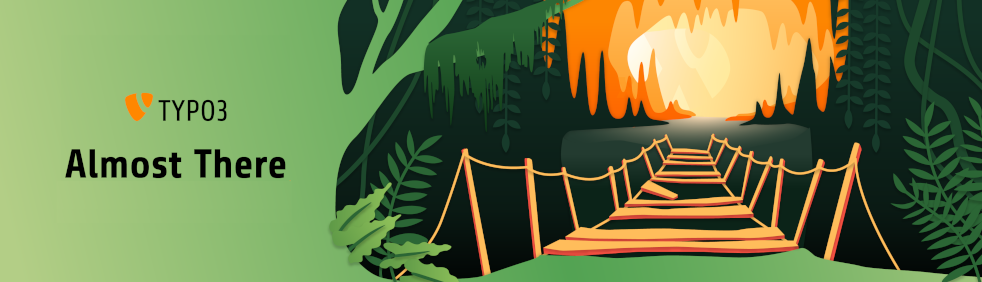
\includegraphics[width=0.95\linewidth]{Introduction/typo3-v10-3-banner.png}
	\end{figure}

\end{frame}

% ------------------------------------------------------------------------------
% TYPO3 Version 10.3 - Executive Summary

\begin{frame}[fragile]
	\frametitle{Uvod}
	\framesubtitle{Rezime}

	\small
		Kao poslednja brza objava iz životnog ciklusa, TYPO3 verzija 10.3 je takozvana
		verzija "\href{https://typo3.org/article/land-ho-feature-freeze-ahead}{zamrzavanje funkcionalnosti}".
		Ovo znači da više neće biti novih funkcionalnosti do LTS verzije u aprilu,
		tako da je ceo tim fokusiran na testiranje, sredjivanje i prečišćavanje koda.

		\vspace{0.2cm}

		Postoje odredjeni izuzetci za mala unapredjenja, koja su zapravo završavanje funkcionalnosti
		koje su započete u prethodnim brzim objavama verzije 10.

		\vspace{0.2cm}

		Ukoliko ste Vi programer proširenja, molimo Vas da objavite verzije koje su kompatibilne sa
		verzijom 10. Ovo će olakšati TYPO3 zajednici da prihvati TYPO3 v10 čim se objavi LTS verzija.

		\vspace{0.2cm}

		Poslednja važna stvar: ne zaboravite da se priključite
		\href{https://typo3.org/community/events/v10-parties}{žurci objave}
		ili sami organizujete istu!

	\normalsize

\end{frame}

% ------------------------------------------------------------------------------
% System Requirements

\begin{frame}[fragile]
	\frametitle{Uvod}
	\framesubtitle{Sistemski zahtevi}

	\begin{itemize}
		\item PHP verzija 7.2, 7.3 ili 7.4
		\item PHP podešavanja:

			\begin{itemize}
				\item \texttt{memory\_limit} >= 256M
				\item \texttt{max\_execution\_time} >= 240s
				\item \texttt{max\_input\_vars} >= 1500
				\item opcija \texttt{-}\texttt{-disable-ipv6} \underline{ne sme} se koristiti
			\end{itemize}

		\item Većina DB servera koji rade sa \textbf{Doctrine DBAL} rade takodje i sa TYPO3.
			Testirani DB serveri su:
	\end{itemize}

	\begin{figure}
		
\includegraphics[width=0.80\linewidth]{Introduction/logo-databases.png}
	\end{figure}

\end{frame}

% ------------------------------------------------------------------------------
% Development, Release, and Maintenance Timeline

\begin{frame}[fragile]
	\frametitle{Uvod}
	\framesubtitle{Razvoj, objavljivanje i vreme održavanja}

	\textbf{TYPO3 v10}

	\begin{figure}
		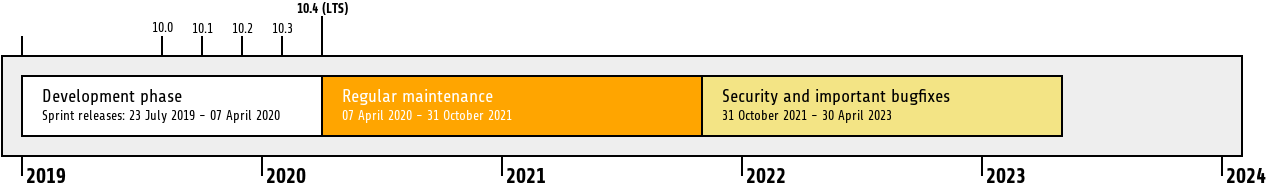
\includegraphics[width=1\linewidth]{Introduction/typo3-v10-lifecycle.png}
	\end{figure}

	\textbf{Produženo vreme podrške}\newline
	\smaller
		\href{https://typo3.com}{TYPO3 GmbH} nudi dodatne opcije za podršku za
		TYPO3 v10 LTS čak i posle 30. aprila 2023. za dodatne dve godine.
	\normalsize

\end{frame}

% ------------------------------------------------------------------------------
% TYPO3 v10 Roadmap

\begin{frame}[fragile]
	\frametitle{Uvod}
	\framesubtitle{TYPO3 v10 plan}

	Predvidjeni datumi objavljivanja i njihov osnovni fokus:

	\begin{itemize}

		\item v10.0 \tabto{1.1cm}23. jul 2019.\tabto{3.4cm}Otvaranje puta za uzbudljive nove koncepte i API-je
		\item v10.1 \tabto{1.1cm}01. okt. 2019.\tabto{3.4cm}Unapredjenje routing-a i upravljanje sajtom v2
		\item v10.2 \tabto{1.1cm}03. dec. 2019.\tabto{3.4cm}Fluid/Rendering Engine unapredjenja
		\item
			\begingroup
				\color{typo3orange}
				v10.3 \tabto{1.1cm}25. feb. 2020\tabto{3.4cm}Zamrzavanje funkcionalnosti
			\endgroup
		\item v10.4 \tabto{1.1cm}21. Apr. 2020\tabto{3.4cm}LTS objava (objava sa dugoročnom podrškom)

	\end{itemize}

	\vspace{0.6cm}
	\smaller
		\url{https://typo3.org/article/typo3-v10-roadmap/}\newline
		\url{https://typo3.org/article/typo3-v10-safe-and-sound/}
	\normalsize

\end{frame}

% ------------------------------------------------------------------------------
% Installation

\begin{frame}[fragile]
	\frametitle{Uvod}
	\framesubtitle{Instalacija}

	\begin{itemize}
		\item Zvanična \textit{klasična} procedura za instalaciju na Linux/Mac OS X
			(DocumentRoot na primer \texttt{/var/www/site/htdocs}):
\begin{lstlisting}
$ cd /var/www/site
$ wget --content-disposition get.typo3.org/10.3
$ tar xzf typo3_src-10.3.0.tar.gz
$ cd htdocs
$ ln -s ../typo3_src-10.3.0 typo3_src
$ ln -s typo3_src/index.php
$ ln -s typo3_src/typo3
$ touch FIRST_INSTALL
\end{lstlisting}

		\item Simbolički linkovi (Symbolic links) na Microsoft Windows:

			\begin{itemize}
				\item Koristiti \texttt{junction} za Windows XP/2000
				\item Koristiti \texttt{mklink} za Windows Vista i Windows 7 i novije
			\end{itemize}

	\end{itemize}
\end{frame}

% ------------------------------------------------------------------------------
% Installation using composer

\begin{frame}[fragile]
	\frametitle{Uvod}
	\framesubtitle{Instalacija korišćenjem \texttt{composer-a}}

	\begin{itemize}
		\item Instalacija korišćenjem \textit{composer-a} na Linux/Mac OS X i Windows 10:
\begin{lstlisting}
$ cd /var/www/site/
$ composer create-project typo3/cms-base-distribution typo3v10 ^10.3
\end{lstlisting}

		\item Alternativno, napravite Vaš \texttt{composer.json} fajl i pokrenite:
\begin{lstlisting}
$ composer install
\end{lstlisting}

			Više detalja i primer \texttt{composer.json} fajla možete skinuti sa:
			\smaller
				\href{https://composer.typo3.org}{https://composer.typo3.org}
			\normalsize

	\end{itemize}
\end{frame}

% ------------------------------------------------------------------------------
